\documentclass[a4paper,12pt]{article}

\usepackage{mystyle}
\usepackage{gensymb}


\usepackage{scalerel}
\usepackage{stackengine}

\graphicspath{ {images/} }


% https://tex.stackexchange.com/questions/5461/is-it-possible-to-change-the-size-of-an-arrowhead-in-tikz-pgf
\usetikzlibrary{arrows.meta}


\DeclareMathOperator{\Image}{Im}
\definecolor{violet}{RGB}{148, 0, 211}
\definecolor{green}{RGB}{0, 153, 0}
\definecolor{orange}{RGB}{255, 153, 0}
\definecolor{blue}{RGB}{31, 117, 254}


% https://tex.stackexchange.com/a/101138/135045

\newcommand\widesim[1]{\ThisStyle{%
  \setbox0=\hbox{$\SavedStyle#1$}%
  \stackengine{-.1\LMpt}{$\SavedStyle#1$}{%
    \stretchto{\scaleto{\SavedStyle\mkern.2mu\sim}{.5150\wd0}}{.6\ht0}%
  }{O}{c}{F}{T}{S}%
}}

\newcommand{\BigMiddleThree}{\;\left|\vphantom{\begin{pmatrix} 0\\0\\0 \end{pmatrix}}\right.\;}
\newcommand{\BigMiddleFour}{\;\left|\vphantom{\begin{pmatrix} 0\\0\\0\\0 \end{pmatrix}}\right.\;}


% https://tex.stackexchange.com/questions/63531/how-to-write-quotation-marks-in-math-environment
\DeclareMathSymbol{\mlq}{\mathord}{operators}{``}
\DeclareMathSymbol{\mrq}{\mathord}{operators}{`'}


\DeclareMathOperator{\Imag}{Im}


% https://tex.stackexchange.com/questions/544453/undefined-control-sequence-after-paragraph
\renewcommand{\paragraph}[1]{\noindent\textbf{#1}\quad}



% https://tex.stackexchange.com/questions/4813/extendible-equals-sign
\makeatletter
\newcommand*{\Relbarfill@}{\arrowfill@\Relbar\Relbar\Relbar}
\newcommand*{\xeq}[2][]{\ext@arrow 0055\Relbarfill@{#1}{#2}}
\makeatother



% https://tex.stackexchange.com/questions/279100/typeset-the-shrug-%C2%AF-%E3%83%84-%C2%AF-emoji
\newcommand{\shrug}[1][]{%
\begin{tikzpicture}[baseline,x=0.8\ht\strutbox,y=0.8\ht\strutbox,line width=0.125ex,#1]
  \def\arm{(-2.5,0.95) to (-2,0.95) (-1.9,1) to (-1.5,0) (-1.35,0) to (-0.8,0)};
  \draw \arm;
  \draw[xscale=-1] \arm;
  \def\headpart{(0.6,0) arc[start angle=-40, end angle=40,x radius=0.6,y radius=0.8]};
  \draw \headpart;
  \draw[xscale=-1] \headpart;
  \def\eye{(-0.075,0.15) .. controls (0.02,0) .. (0.075,-0.15)};
  \draw[shift={(-0.3,0.8)}] \eye;
  \draw[shift={(0,0.85)}] \eye;
  % draw mouth
  \draw (-0.1,0.2) to [out=15,in=-100] (0.4,0.95); 
\end{tikzpicture}}




\author{Алексеев Василий}


\title{
    Семинар 6 + 5\\\medskip
    \Large Линейные преобразования\\евклидовых пространств.\\\medskip
    ``Diag 1.2''
}
\date{21 апреля + 25 апреля 2022}


\begin{document}
  \maketitle
  
  \tableofcontents

  \thispagestyle{empty}
  
  \newpage
  
  
  
  \vspace*{\fill}
  
  \noindent
  \emph{
    Жирным шрифтом обозначаются как векторы линейного пространства, так и их координатные столбцы в выбранном базисе.
    При этом и векторы, и их координатные столбцы обозначаются, как правило, одинаковыми буквами.
    Например, $\bds x \hm\in X$ (вектор) и $\bds x \hm\in \RR^{\dim X}$ (координатный столбец).
    Таким образом, смысл зависит от контекста
  } \shrug
  
  \vspace*{\fill}
  
  \thispagestyle{empty}
  
  \newpage
  
  
  \pagenumbering{arabic}


  \section{Самосопряжённые преобразования}
  
  \subsection{\# 29.19(7)}
  \label{p29-19}
  
  Преобразование $\phi\hm\colon X \hm\to X$, где $X$~---~евклидово пространство, задано в \emph{ортонормированном базисе} матрицей:
  \[
    A = \begin{pmatrix}
      1 & -4 & 1\\
      -4 & 16 & -4\\
      1 & -4 & 1
    \end{pmatrix}
  \]
  Надо найти ортонормированный базис из собственных векторов преобразования $\phi$, матрицу перехода $S$ к этому базису, и матрицу преобразования $\phi$ в указанном базисе.
  
  \begin{solution}
  
  Найдём \textbf{собственные значения} преобразования $\phi$.
  Характеристическое уравнение:
  \[
    \det (A - \lambda E) = 0
  \]
  \[
    \begin{vmatrix}
      1 - \lambda & -4 & 1\\
      -4 & 16 - \lambda & -4\\
      1 & -4 & 1 - \lambda
    \end{vmatrix} = \ldots = \lambda^2 (18 - \lambda) = 0
  \]
  
  Корни характеристического уравнения:
  \[
    \left[
      \begin{aligned}
        &\lambda = 0\quad \mbox{(кратность $2$)}\\
        &\lambda = 18
      \end{aligned}
    \right.
  \]
  Видно, что \emph{все корни характеристического уравнения вещественные}, поэтому они же~---~и собственные значения преобразования $\phi$.
  
  При этом то, что $\lambda \hm= 0$~---~собственное значение, можно бы было (стоило бы) заметить и в самом начале, ведь у матрицы $A$ строки уже линейно зависимы (первая и третья совпадают), то есть $\det(A \hm- \lambda E)|_{\lambda = 0} \hm= 0$.
  
  \medskip
  
  Найдём \textbf{собственные векторы} преобразования $\phi$ (максимальную линейно независимую систему собственных векторов).
  При $\lambda \hm= 0$ получаем следующее уравнение для поиска собственных векторов:
  \[
    A \bds x = \lambda \bds x
  \]
  \[
    (A - \lambda E) \bds x = \bds 0
  \]
  \[
    \begin{pmatrix}
      1 & -4 & 1\\
      -4 & 16 & -4\\
      1 & -4 & 1
    \end{pmatrix} \begin{pmatrix}
      x_1 \\ x_2 \\ x_3
    \end{pmatrix} = \bds 0
  \]
  
  Последнее матричное уравнение равносильно одному скалярному уравнению
  \[
    x_1 - 4 x_2 + x_3 = 0
  \]
  
  Из которого можно выразить $x_1$ через $x_2$ и $x_3$:
  \[
    x_1 = 4 t_1 - t_2,\quad x_2 = t_1 \in \RR,\quad x_3 = t_2 \in \RR
  \]
  
  Тогда общее решение $A \bds x \hm= \bds 0$ (произвольный вектор из собственного подпространства $\Ker (A \hm- \lambda E)|_{\lambda = 0}$) можно выписать в виде:
  \[
    \bds x = \begin{pmatrix}
      4 t_1 - t_2\\
      \hphantom{4} t_1 \hphantom{- t_2}\\
      \hphantom{4 t_1 -} t_2
    \end{pmatrix}
    = t_1 \cdot \begin{pmatrix}
      4 \\ 1 \\ 0
    \end{pmatrix}
    + t_2 \cdot \begin{pmatrix}
      -1 \\ 0 \\ 1
    \end{pmatrix}
  \]
  
  Видно, что в качестве базиса в собственном подпространстве $\phi$, соответствующем собственному значению $\lambda \hm= 0$ (максимальная линейно независимая система собственных векторов для $\lambda \hm= 0$) можно взять векторы:
  \[
    \bds x_1 = \begin{pmatrix}
      4 \\ 1 \\ 0
    \end{pmatrix},\quad
    \bds x_2 = \begin{pmatrix}
      -1 \\ 0 \\ 1
    \end{pmatrix}
  \]
  
  (Не лишним будет на всякий случай проверить, что $A \bds x_1 \hm= \bds 0$ и $A \bds x_2 \hm= \bds 0$.)
  
  \medskip
  
  Теперь найдём собственные векторы для $\lambda \hm= 18$.
  Уравнение, определяющее соответствующее собственное подпространство:
  \[
    \begin{pmatrix}
      -17 & -4 & 1\\
      -4 & -2 & -4\\
      1 & -4 & -17
    \end{pmatrix} \begin{pmatrix}
      x_1 \\ x_2 \\ x_3
    \end{pmatrix} = \bds 0
  \]
  
  Упростим матрицу соответствующей однородной системы:
  \[
    \begin{pmatrix}
      \bds{-17} & -4 & 1\\
      \bds{-4} & -2 & -4\\
      1 & -4 & -17
    \end{pmatrix}
    \sim \begin{pmatrix}
      0 & -72 & -288\\
      0 & -18 & -72\\
      1 & -4 & -17
    \end{pmatrix}
    \sim \begin{pmatrix}
      0 & \bds{1} & 4\\
      0 & 1 & 4\\
      1 & \bds{-4} & -17
    \end{pmatrix}
    \sim \begin{pmatrix}
      0 & 0 & 0\\
      0 & 1 & 4\\
      1 & 0 & -1
    \end{pmatrix}
  \]
  
  То есть упрощённая система будет выглядеть следующим образом:
  \[
    \left\{
      \begin{aligned}
        &\hphantom{x_1 +} x_2 + 4 x_3 = 0\\
        &x_1 \hphantom{+ x_2} - \hphantom{4} x_3 = 0
      \end{aligned}
    \right.;\quad
    \left\{
      \begin{aligned}
        &x_2 = -4 x_3\\
        &x_1 = x_3
      \end{aligned}
    \right.
  \]
  
  Общее решение:
  \[
    \bds x = \begin{pmatrix}
      t \\ -4t \\ t
    \end{pmatrix}
    = t \cdot \begin{pmatrix}
      1 \\ -4 \\ 1
    \end{pmatrix},\quad t \in \RR
  \]
  
  Базис в собственном подпространстве (один вектор):
  \[
    \bds x_3 = \begin{pmatrix}
      1 \\ -4 \\ 1
    \end{pmatrix}
  \]
  
  (На всякий случай убеждаемся, что $A \bds x_3 = 18 \bds x_3$.)
  
  \medskip
  
  Таким образом, мы нашли \emph{базис из собственных векторов} преобразования $\phi$:
  \begin{equation}\label{p29-19:basis}
    \{\bds x_1, \bds x_2, \bds x_3\} = \left\{
      \begin{pmatrix}
        4 \\ 1 \\ 0
      \end{pmatrix},
      \begin{pmatrix}
        -1 \\ 0 \\ 1
      \end{pmatrix},
      \begin{pmatrix}
        1 \\ -4 \\ 1
      \end{pmatrix}
    \right\}
  \end{equation}
  
  \medskip
  
  Теперь проведём \textbf{ортогонализацию} системы векторов (\ref{p29-19:basis}).
  Исходный базис ортонормированный, поэтому скалярное произведение между векторами $\bds x \hm= (x_1, \ldots, x_n)^T$ и $\bds y \hm= (y_1, \ldots, y_n)^T$ считается как
  \[
    (\bds x, \bds y) = x_1 y_1 + \ldots + x_n y_n
  \]
  
  Видно, что $(\bds x_1, \bds x_3) \hm= 4 \hm- 4 \hm+ 0 \hm= 0$.
  Так же, как и $(\bds x_2, \bds x_3) \hm= -1 \hm+ 0 \hm+ 1 \hm= 0$.
  
  То есть \emph{собственные векторы, соответствующие различным собственным значениям преобразования $\phi$, ортогональны}.
  
  Остаётся ``поправить'' подсистему $\{\bds x_1, \bds x_2\}$, потому что $(\bds x_1, \bds x_2) \hm= -4 \hm{\not=} 0$.
  Вычтем, например, из $\bds x_1$ его ортогональную проекцию на $\bds x_2$:
  \[
    \bds x_1' = \bds x_1 - \frac{(\bds x_1, \bds x_2)}{|\bds x_2|} \cdot \frac{\bds x_2}{|\bds x_2|}
    = \begin{pmatrix}4 \\ 1 \\ 0\end{pmatrix} + 2 \begin{pmatrix}-1 \\ 0 \\ 1\end{pmatrix}
    = \begin{pmatrix}2 \\ 1 \\ 2\end{pmatrix}
  \]
  где было использовано, что $|\bds x_2|^2 \hm= 1 \hm+ 0 \hm+ 1 \hm= 2$.
  
  Убеждаемся, что $(\bds x_1', \bds x_2) \hm= -2 \hm+ 0 \hm+ 2 \hm= 0$.
  Так как мы считали $\bds x_1'$ как линейную комбинацию $\bds x_1$ и $\bds x_2$, то $(\bds x_1', \bds x_3) \hm= 0$ (можно не проверять ортогональность $\bds x_3$; ну, или можно проверить, но стоит понимать, что ничего удивительного в сохранении ортогональности $\bds x_1'$ и $\bds x_3$ нет).
  Получили ортогональную систему из собственных векторов преобразования $\phi$?..
  А остался ли вектор $\bds x_1'$ собственным для $\lambda \hm= 0$?
  Да, ведь он получен как линейная комбинация $\bds x_1$ и $\bds x_2$~---~векторов из собственного подпространства $\Ker(A \hm- \lambda E)|_{\lambda = 0}$, а потому $\bds x_1'$ тоже лежит в указанном собственном подпространстве ($A \bds x_1' \hm= \bds 0$).
  
  Итого, помимо просто базиса из собственных векторов, для преобразования $\phi$ \emph{существует ортогональный базис из собственных векторов}:
  \begin{equation}\label{p29-19:orto-basis}
    \{\bds x_1', \bds x_2, \bds x_3\} = \left\{
      \begin{pmatrix}
        2 \\ 1 \\ 2
      \end{pmatrix},
      \begin{pmatrix}
        -1 \\ 0 \\ 1
      \end{pmatrix},
      \begin{pmatrix}
        1 \\ -4 \\ 1
      \end{pmatrix}
    \right\}
  \end{equation}
  
  \medskip
  
  Чтобы \textbf{нормировать} базис, надо теперь просто поделить все векторы (\ref{p29-19:orto-basis}) на их модули:
  \[
    \left\{
      \begin{aligned}
        &|\bds x_1'| = \sqrt{4 + 1 + 4} = 3\\
        &|\bds x_2| = \sqrt{1 + 1} = \sqrt{2}\\
        &|\bds x_3| = \sqrt{1 + 16 + 1} = 3 \sqrt{2}
      \end{aligned}
    \right.
  \]
  
  Имеем следующий ортонормированный базис из собственных векторов:
  \begin{equation}\label{p29-19:ortonorm-basis}
    \{\bds x_1'', \bds x_2'', \bds x_3''\} = \left\{
      \frac{1}{3} \begin{pmatrix}
        2 \\ 1 \\ 2
      \end{pmatrix},
      \frac{1}{\sqrt{2}} \begin{pmatrix}
        -1 \\ 0 \\ 1
      \end{pmatrix},
      \frac{1}{3 \sqrt{2}} \begin{pmatrix}
        1 \\ -4 \\ 1
      \end{pmatrix}
    \right\}
  \end{equation}
  
  \medskip
  
  Матрица перехода $S$ от старого ортонормированного базиса в новому $\{\bds x_1'', \bds x_2'', \bds x_3''\}$~---~это матрица, столбцы которой есть компоненты новых базисных векторов в старом базисе.
  То есть матрица $S$ получается просто объединением столбцов (\ref{p29-19:ortonorm-basis}) в матрицу:
  \[
    S = \begin{pmatrix}
      2 / 3 & -1 / \sqrt{2} & 1 / \left(3 \sqrt{2}\right)\\
      1 / 3 & 0             & -4 / \left(3 \sqrt{2}\right)\\
      2 / 3 & 1 / \sqrt{2}  & 1 / \left(3 \sqrt{2}\right)
    \end{pmatrix}
  \]
  
  Можно заметить, что $S^T S \hm= E$, то есть матрица перехода $S$ ортогональная.
  Это потому, что $S$~---~матрица перехода от \emph{одного ортонормированного} базиса к \emph{другому ортонормированному} базису.
  Например,
  \[
    (S^T S)_{12} = \bds x_1''^T \bds x_2'' \xeq{\mbox{\footnotesize старый ОНБ}} (\bds x_1'', \bds x_2'') \xeq{\mbox{\footnotesize новый ОНБ}} 0
  \]
  
  \medskip
  
  Чтобы найти матрицу $A'$ преобразования $\phi$ в новом базисе, можно воспользоваться либо тем, что новый базис~---~это базис из собственных векторов (например, в новом базисе $\bds x_1''$ имеет координаты $(1, 0, 0)^T$, поэтому образ $\bds x_1''$ будет просто первым столбцом $A'$, а это $\lambda \bds x_1''|_{\lambda = 0}$, так как вектор $\bds x_1''$~---~собственный, соответствующий $\lambda \hm= 0$), то есть
  \[
    A' = \begin{pmatrix}
      0 & 0 & 0\\
      0 & 0 & 0\\
      0 & 0 & 18
    \end{pmatrix}
  \]
  
  Либо тем, что уже известна матрица $S$ перехода от старого базиса к новому:
  \[
    A' = S^{-1} A S \xeq{S^T S = E} S^T A S = \ldots = \begin{pmatrix}
      0 & 0 & 0\\
      0 & 0 & 0\\
      0 & 0 & 18
    \end{pmatrix}
  \]
  
  Первый способ, очевидно, побыстрее :)
  Но вторым, с матрицей $S$, можно хотя бы проверить, что всё в порядке.
  Если только не ошибиться в процессе самой проверки :)
  \end{solution}
  
  
  \subsection{Самосопряжённые преобразования}
  
  Пусть есть линейное преобразование $\phi\hm\colon X \hm\to X$ \emph{евклидова} пространства $X$ (то есть пространство, в котором выбрано скалярное произведение $(\cdot, \cdot)$).
  Тогда преобразованием, \emph{сопряжённым} преобразованию $\phi$, называется преобразование $\phi^*\hm\colon X \hm\to X$, такое что
  \begin{equation}\label{eq:adjoint}
    \boxed{\bigl(\phi(\bds x), \bds y\bigr) = \bigl(\bds x, \phi^*(\bds y)\bigr),\quad \forall \bds x, \bds y \in X}
  \end{equation}
  
  Пусть $e$~---~базис в $X$.
  Пусть матрица $A$~---~матрица преобразования $\phi$ в этом базисе, $A^*$~---~матрица сопряжённого преобразования $\phi^*$, а $\Gamma$~---~матрица Грама базиса.
  Тогда левую часть соотношения (\ref{eq:adjoint}) можно переписать в таком виде:
  \[
    (\phi(\bds x), \bds y) = (A \bds x)^T \Gamma \bds y = \bds x^T \cdot A^T \Gamma \cdot \bds y
  \]
  
  А правая часть (\ref{eq:adjoint}) будет выглядеть как
  \[
    (\bds x, \phi^*(\bds y)) = \bds x^T \Gamma (A^* \bds y) = \bds x^T \cdot \Gamma A^* \cdot \bds y
  \]
  
  Так как (\ref{eq:adjoint}) верно для произвольной пары $(\bds x, \bds y)$, то равны ``матрицы посередине'':
  \begin{equation}
    \boxed{A^T \Gamma = \Gamma A^*}
  \end{equation}
  
  Так как $\Gamma$~---~матрица Грама, то можно соотношение между матрицами исходного и сопряжённого преобразований переписать в таком виде:
  \[
    A^* = \Gamma^{-1} A^T \Gamma
  \]
  
  В \emph{ортонормированном} базисе матрица сопряжённого преобразования оказывается равной
  \[
    A^* = A^T\quad \mbox{(ОНБ)}
  \]
  
  \medskip
  
  Преобразование $\phi$ евклидова пространства $X$ называется \emph{самосопряжённым}, если оно совпадает со своим сопряжённым $\phi^*$, то есть $\phi(\bds x) \hm= \phi^*(\bds x)$, $\forall \bds x \hm\in X$, или:
  \begin{equation}\label{eq:self-adjoint-def}
    \boxed{
      \bigl(\phi(\bds x), \bds y\bigr) = \bigl(\bds x, \phi(\bds y)\bigr),\quad \forall \bds x, \bds y \in X
    }
  \end{equation}
  
  Матрица самосопряжённого преобразования удовлетворяет соотношению:
  \begin{equation}\label{eq:self-adjoint}
    \boxed{A^T \Gamma = \Gamma A}
  \end{equation}
  
  В ортонормированном базисе:
  \[
    A = A^T\quad \mbox{(ОНБ)}
  \]
  
  \medskip
  
  Отметим несколько свойств самосопряжённых преобразований в контексте собственных значений и собственных векторов.
  
  \begin{theorem}\label{theo:real-roots}
    Все корни характеристического уравнения самосопряжённого преобразования вещественные\footnote{При этом интересно, что корни характеристического уравнения~---~это характеристика именно преобразования, а самосопряжённость связана с конкретным скалярным произведением.}.
  \end{theorem}
  
  \begin{example}
    Убедимся в этом на примере самосопряжённого преобразования двумерного пространства, заданного матрицей в ортонормированном базисе (симметричной).
    Пусть матрица преобразования $A \hm= \left(\begin{smallmatrix}a & b\\ b & c\end{smallmatrix}\right)$.
    Тогда характеристическое уравнение:
    \[
      \det(A - \lambda E) = \begin{vmatrix}
        a - \lambda & b\\
        b & c - \lambda
      \end{vmatrix} = 0
    \]
    \[
      \lambda^2 - (a + c) \lambda + (b^2 + ac) = 0
    \]
    
    Дискриминант $(a \hm+ c)^2 \hm- 4(b^2 \hm+ ac) \hm= (a \hm- c)^2 \hm+ b^2 \hm\geq 0$, поэтому оба корня $\lambda_{1, 2}$ действительные.
  \end{example}
  
  Пусть теперь $\lambda_1$ и $\lambda_2$~---~различные собственные значения самосопряжённого преобразования $\phi$.
  Пусть $\bds x_1$ и $\bds x_2$~---~соответственные собственные векторы.
  Тогда, с одной стороны,
  \[
    (\phi(\bds x_1), \bds x_2) = (\lambda_1 \bds x_1, \bds x_2) = \lambda_1 (\bds x_1, \bds x_2)
  \]
  
  С другой стороны,
  \[
    (\phi(\bds x_1), \bds x_2) = (\bds x_1, \phi(\bds x_2)) = (\bds x_1, \lambda_2 \bds x_2) = \lambda_2 (\bds x_1, \bds x_2)
  \]
  
  Отсюда получаем, что
  \[
    \lambda_1 (\bds x_1, \bds x_2) = \lambda_2 (\bds x_1, \bds x_2) \Leftrightarrow (\lambda_2 - \lambda_1) (\bds x_1, \bds x_2) = 0
  \]
  
  Но собственные значения по условию различны, поэтому $(\bds x_1, \bds x_2) \hm= 0$.
  То есть \emph{собственные векторы, соответствующие различным собственным значениям самосопряжённого преобразования, ортогональны}\footnote{Собственные векторы ненулевые по определению, поэтому можно говорить именно об ортогональности (``угол между векторами равен $90$ градусам'').}.
  
  \begin{theorem}
    Для самосопряжённого преобразования $\phi$ найдётся ортонормированный базис из собственных векторов.
  \end{theorem}
  
  То есть, с одной стороны, найдётся базис из собственных векторов (даже если у характеристического уравнения будут кратные корни~---~каждому собственному значению будет соответствовать собственное подпространство той же размерности, что и кратность собственного значения как корня характеристического уравнения).
  С другой стороны, базис можно будет ортогонализировать.
  
  \begin{example}
    Преобразование, рассмотренное в (\ref{p29-19}), было задано симметричной матрицей в ортонормированном базисе.
    То есть преобразование было самосопряжённым.
    Поэтому для него точно можно было найти ортонормированный базис из собственных векторов.
  \end{example}
  
  \medskip
  
  Итак, свойство самосопряжённости связано со скалярным произведением, выбранным в пространстве $X$.
  Проверим, что матричное соотношение (\ref{eq:self-adjoint}), хотя матрицы и зависят от выбора базиса, выполняется и при \emph{смене базиса} (очевидно, должно выполняться, ведь в определении самосопряжённого преобразования (\ref{eq:self-adjoint-def}) никакой конкретный базис не участвовал).
  Пусть $e$~---~``старый'' базис, а $e' \hm= e S$~---~``новый'' базис.
  Тогда матрица преобразования в новом базисе $A' \hm= S^{-1} A S$, матрица Грама нового базиса $\Gamma' \hm= S^T \Gamma S$, и соотношение (\ref{eq:self-adjoint}), которое хотим проверить для новых матриц:
  \begin{equation*}
  \begin{split}
    A'^T \Gamma' = \Gamma' A'
    &\Leftrightarrow (S^{-1} A S)^T (S^T \Gamma S) = (S^T \Gamma S) (S^{-1} A S)\\
    &\Leftrightarrow S^T A^T \Gamma S = S^T \Gamma A S
    \Leftrightarrow A^T \Gamma = \Gamma A
  \end{split}
  \end{equation*}
  
  То есть, да, от выбора базиса самосопряжённость не зависит.
  
  
  
  \subsection{\# 29.14(2, 3)}
  
  Может ли самосопряжённое преобразование в каком-то базисе иметь матрицу $A_2$ или $A_3$, где
  \[
    A_2 = \begin{pmatrix}
      0 & -1\\
      1 & -1
    \end{pmatrix},\quad
    A_3 = \begin{pmatrix}
      5 & 14\\
      6 & 13
    \end{pmatrix}
  \]
  
  \begin{solution}
    То есть скалярное произведение $(\cdot, \cdot)$ задано, можно только пытаться найти подходящий базис.
    
    Рассмотрим матрицу $A_2$.
    Её характеристическое уравнение:
    \[
      \det(A_2 - \lambda E) = \begin{vmatrix}
        -\lambda & -1\\
        1 & -1 - \lambda
      \end{vmatrix} = \lambda^2 + \lambda + 1 = 0
    \]
    
    Очевидно, нет действительных корней.
    Поэтому преобразование с матрицей $A_2$ не может быть самосопряжённым (\ref{theo:real-roots}).
    
    \medskip
    
    Характеристическое уравнение для матрицы $A_3$:
    \[
      \det(A_3 - \lambda E) = \begin{vmatrix}
        5 - \lambda & 14\\
        6 & 13 - \lambda
      \end{vmatrix} = \lambda^2 - 18\lambda - 19 = 0
    \]
    \[
      \left[
        \begin{aligned}
          &\lambda = -1\\
          &\lambda = 19
        \end{aligned}
      \right.
    \]
    
    То есть у преобразования $\phi$ с матрицей $A_3$ точно есть базис из собственных векторов.
    \emph{Если} получится найти \emph{ортонормированный} базис из собственных векторов, то в этом базисе матрица $\phi$ будет диагональной, а потому преобразование $\phi$ будет самосопряжённым (как преобразование с симметричной матрицей в ортонормированном базисе).
    
    Будут ли собственные векторы ортогональны или нет~---~очевидно, как раз зависит от выбора базиса.
    Найдём собственные векторы:
    \[
      A_3 \bds x = \lambda \bds x|_{\lambda = -1} \Rightarrow \bds x_1 = (7, -3)^T
    \]
    \[
      A_3 \bds x = \lambda \bds x|_{\lambda = 19} \Rightarrow \bds x_2 = (1, 1)^T
    \]
    
    Пусть матрица Грама искомого базиса равна $\Gamma \hm= \left(\begin{smallmatrix}a & b\\ b & c\end{smallmatrix}\right)$, $a \hm> 0$, $ac \hm- b^2 \hm> 0$.
    Тогда скалярное произведение собственных векторов будет равно
    \[
      (\bds x_1, \bds x_2) = \bds x_1^T \Gamma \bds x_2
      = \begin{pmatrix}
        7 & -3
      \end{pmatrix} \begin{pmatrix}
        a & b\\
        b & c
      \end{pmatrix}
      \begin{pmatrix}
        1\\ 1
      \end{pmatrix}
    \]
    
    Хотим найти базис, такой что $(\bds x_1, \bds x_2) \hm= 0$.
    Приходим к условию на элементы матрицы Грама:
    \[
      7a + 7b - 3b - 3c = 7a + 4b - 3c = 0
    \]
    
    Итого, объединяя условия, связанные с положительной определённостью матрицы Грама, сводим поиск базиса к поиску решения следующей системы с ограничениями:
    \[
      \left\{
        \begin{aligned}
          &7a + 4b - 3c = 0\\
          &a > 0\\
          &ac - b^2 > 0
        \end{aligned}
      \right.
    \]
    
    Равенство задаёт плоскость в пространстве $(a, b, c)$, первое неравенство~---~полупространство, второе~---~``внутренность'' конуса.
    В качестве решения можно взять, например, следующее:
    \[
      a = 3,\quad b = 0,\quad c = 7
    \]
    
    То есть искомый базис~---~такой, матрица Грама которого равна, например, $\left(\begin{smallmatrix}3 & 0\\ 0 & 7\end{smallmatrix}\right)$.
    
    \medskip
    
    Для поиска матрицы Грама базиса можно бы было идти другим путём.
    Матрица самосопряжённого преобразования удовлетворяет условию (\ref{eq:self-adjoint}):
    \[
      A_3^T G = G A_3
    \]
    
    Если снова обозначить матрицу Грама как $\Gamma \hm= \left(\begin{smallmatrix}a & b\\ b & c\end{smallmatrix}\right)$, $a \hm> 0$, $ac \hm- b^2 \hm> 0$, то получаем
    \[
      \begin{pmatrix}
        5 & 6\\
        14 & 13
      \end{pmatrix}
      \begin{pmatrix}
        a & b\\
        b & c
      \end{pmatrix}
      = \begin{pmatrix}
        a & b\\
        b & c
      \end{pmatrix}
      \begin{pmatrix}
        5 & 14\\
        6 & 13
      \end{pmatrix}
    \]
    \[
      \begin{pmatrix}
        5a + 6b & 5b + 6c\\
        14a + 13b & 14b + 13c
      \end{pmatrix}
      = \begin{pmatrix}
        5a + 6b & 14a + 13b\\
        5b + 6c & 14b + 13c
      \end{pmatrix}
    \]
    
    Что равносильно
    \[
      14a + 13b = 5b + 6c \Leftrightarrow 7 a + 4 b - 3 c = 0
    \]
    
    Получили то же, что и в прошлый раз (когда требовали ортогональность собственных векторов).
    
    \medskip
    
    \emph{P.S. (``Объяснение'' на пальцах)}
    
    Итого, мы проверили на конкретном примере, что если на плоскости даны в координатах два неколлинеарных вектора, то можно найти базис, в котором векторы с такими координатами будут перпендикулярны (скалярное произведение фиксировано).
    Можно себе это представить как ``преобразование плоскости'': если два вектора неколлинеарны, то можно немного ``сжать-растянуть'' (``повернуть'') всё так, чтоб стали перпендикулярны~(\ref{fig:perp-not-perp}).
    
    \begin{figure}
      \centering
      
      \includegraphics[width=0.5\columnwidth]{perp-not-perp}
      
      \caption{Два вектора с координатами $(1, 0)$ и $(0, 1)$: не перпендикулярны в одном базисе (слева), но перпендикулярны в другом базисе (справа).}
      \label{fig:perp-not-perp}
    \end{figure}
  \end{solution}
  
  
  
  \section{Ортогональные преобразования}
  
  Преобразование $\phi$ евклидова пространства $X$ называется \emph{ортогональным}, если оно сохраняет скалярное произведение.
  То есть если
  \begin{equation}\label{eq:orthogo}
    \boxed{\bigl(\phi(\bds x), \phi(\bds y)\bigr) = (\bds x, \bds y),\quad \forall \bds x, \bds y \in X}
  \end{equation}
  
  Так как скалярное произведение, как симметричная билинейная форма, выражается через соответствующую квадратичную форму, то сохранение скалярного произведения равносильно сохранению длины.
  То есть преобразование ортогональное, если сохраняет длины:
  \[
    \boxed{\bigl(\phi(\bds x), \phi(\bds x)\bigr) = (\bds x, \bds x),\quad \forall \bds x \in X}
  \]
  
  Пусть в $X$ выбран базис $e \hm= (\bds e_1, \ldots, \bds e_n)$.
  Пусть матрица $A$~---~матрица ортогонального преобразования $\phi$ в этом базисе, а $\Gamma$~---~матрица Грама базиса.
  Тогда левую часть (\ref{eq:orthogo}) можно расписать так:
  \[
    (\phi(\bds x), \phi(\bds y)) = (A \bds x)^T \Gamma (A \bds y) = \bds x^T \cdot A^T \Gamma A \cdot \bds y
  \]
  
  Правая часть (\ref{eq:orthogo}):
  \[
    (\bds x, \bds y) = \bds x^T \Gamma \bds y
  \]
  
  Соотношение (\ref{eq:orthogo}) выполнено при произвольных $\bds x$ и $\bds y$, поэтому получаем следующий критерий ортогональности преобразования в матричном виде:
  \[
    \boxed{A^T \Gamma A = \Gamma}
  \]
  
  В ортонормированном базисе:
  \begin{equation}\label{eq:orthogo-matrix-in-onb}
    A^T A = E\quad \mbox{(ОНБ)}
  \end{equation}
  
  То есть \emph{матрица ортогонального преобразования в ортонормированном базисе ортогональна}.
  
  \medskip
  
  Вернёмся к определению ортогонального преобразования~(\ref{eq:orthogo}).
  Ещё один вариант переписать то же самое~---~представив векторы $\bds x$ и $\bds y$ как линейные комбинации базисных.
  Пусть $\bds x \hm= (x_1, \ldots, x_n)$~---~координатный столбец вектора $\bds x$, и $\bds y \hm= (y_1, \ldots, y_n)$~---~координатный столбец вектора $\bds y$.
  Тогда:
  \begin{equation*}
  \begin{split}
    (\bds x, \bds y)
    &= (x_1 \bds e_1 + \ldots + x_n \bds e_n,
        y_1 \bds e_1 + \ldots + y_n \bds e_n)\\
    &= x_1 (\bds e_1, \bds e_1) y_1 + x_1 (\bds e_1, \bds e_2) y_2 + \ldots + x_n (\bds e_n, \bds e_n) y_n\\
    &= \sum_{i, j = 1}^n x_i (\bds e_i, \bds e_j) y_j
  \end{split}
  \end{equation*}
  
  В то же время:
  \begin{equation*}
  \begin{split}
    (\phi(\bds x), \phi(\bds y))
    &= \bigl(\phi(x_1 \bds e_1 + \ldots + x_n \bds e_n),
             \phi(y_1 \bds e_1 + \ldots + y_n \bds e_n)\bigr)\\
    &= \left(x_1 \phi(\bds e_1) + \ldots + x_n \phi(\bds e_n),
             y_1 \phi(\bds e_1) + \ldots + y_n \phi(\bds e_n)\right)\\
    &= x_1 \bigl(\phi(\bds e_1), \phi(\bds e_1)\bigr) y_1
      + x_1 \bigl(\phi(\bds e_1), \phi(\bds e_2)\bigr) y_2
      + \ldots + x_n \bigl(\phi(\bds e_n), \phi(\bds e_n)\bigr) y_n\\
    &= \sum_{i, j = 1}^n x_i \bigl(\phi(\bds e_i), \phi(\bds e_j)\bigr) y_j
  \end{split}
  \end{equation*}
  
  Получаем, что
  \[
    \sum_{i, j = 1}^n x_i (\bds e_i, \bds e_j) y_j = \sum_{i, j = 1}^n x_i \bigl(\phi(\bds e_i), \phi(\bds e_j)\bigr) y_j,\quad \forall \bds x, \bds y \in X
  \]
  
  Это значит, что ортогональность преобразования $\phi$ равносильна также следующему условию:
  \begin{equation}\label{eq:orthogo-basis-paris}
    \boxed{
      \left\{
        \begin{aligned}
          &\bigl(\phi(\bds e_i), \phi(\bds e_j)\bigr) = (\bds e_i, \bds e_j)\\
          &i = 1 \ldots n,\quad j = 1 \ldots n
        \end{aligned}
      \right.
    }
  \end{equation}
  (которое, в свою очередь, можно заметить, приводит к уже ранее полученному $A^T \Gamma A \hm= \Gamma$).
  
  То есть сохранение ортогональным преобразованием скалярного произведения для \emph{любой} пары векторов~---~это то же самое, что сохранение скалярного произведения \emph{лишь} для $n(n\hm-1)/2$ пар базисных векторов.
  
  \medskip
  
  Отметим одно свойство собственных значений ортогонального преобразования $\phi$.
  Пусть $\lambda$~---~собственное значение $\phi$, и $\bds x$~---~соответствующий собственный вектор.
  Тогда
  \[
    (\phi(\bds x), \phi(\bds x)) = (\lambda \bds x, \lambda \bds x) = \lambda^2 (\bds x, \bds x)
    \xeq{\phi\ \mbox{\footnotesize ортогональное}} (\bds x, \bds x)
  \]
  
  То есть $\lambda^2 \hm= 1$.
  Иными словами, \emph{собственные значения ортогонального преобразования по модулю равны единице}.
  
  
  \subsection{\# 29.47(1)}
  
  В евклидовом пространстве $X$ выбран ортонормированный базис.
  Дано преобразование $\phi$, про которое известно, что оно переводит столбцы матрицы $A$ в столбцы матрицы $B$, где
  \[
    A = \begin{pmatrix}
      4 & 2\\
      7 & 1
    \end{pmatrix}
    \quad B = \begin{pmatrix}
      8 & 2\\
      1 & -1
    \end{pmatrix}
  \]
  
  Является ли $\phi$ ортогональным?
  
  \begin{solution}
    Будем считать, что $\phi$ переводит первый столбец $A$ в первый столбец $B$, и второй столбец $A$ во второй столбец $B$ (видимо, так предполагается по условию, хотя вообще это не важно, какой столбец в какой переходит).
    
    Видно, что столбцы $A$ не пропорциональны (так же, как и столбцы $B$).
    Поэтому можно взять векторы $\bds x$ и $\bds y$ с координатными столбцами, совпадающими со столбцами матрицы $A$, в качестве базиса в $X$.
    Тогда столбцы $B$ будут совпадать с координатными столбцами $\phi(\bds x)$ и $\phi(\bds y)$.
    И для проверки ортогональности $\phi$ достаточно проверить (\ref{eq:orthogo-basis-paris}), то есть
    \[
      \left\{
        \begin{aligned}
          &\bigl(\phi(\bds x), \phi(\bds x)\bigr) = (\bds x, \bds x)\\
          &\bigl(\phi(\bds y), \phi(\bds y)\bigr) = (\bds y, \bds y)\\
          &\bigl(\phi(\bds x), \phi(\bds y)\bigr) = (\bds x, \bds y)
        \end{aligned}
      \right.
    \]
    
    Подставляя числа из матриц $A$ и $B$ (и учитывая, что исходный базис ОНБ), получаем:
    \[
      \left\{
        \begin{aligned}
          &16 + 49 = 65 = 64 + 1\\
          &4 + 1 = 5 = 4 + 1\\
          &8 + 7 = 15 = 16 - 1
        \end{aligned}
      \right.
    \]
    
    То есть, да, преобразование $\phi$ является ортогональным.
    
    \medskip
    
    Можно бы было действовать по-другому.
    Пусть $F$~---~матрица преобразования $\phi$.
    Преобразование будет ортогональным, если матрица $F$ ортогональна (\ref{eq:orthogo-matrix-in-onb}) (исходный базис ОНБ).
    По условию сказано, что
    \[
      \left\{
        \begin{aligned}
          &\phi\colon (4, 7)^T \mapsto (8, 1)^T\\
          &\phi\colon (2, 1)^T \mapsto (2, -1)^T
        \end{aligned}
      \right.
    \]
    
    Это можно переписать как
    \[
      \left\{
        \begin{aligned}
          &F \begin{pmatrix}4 \\ 7\end{pmatrix} = \begin{pmatrix}8 \\ 1\end{pmatrix}\\
          &F \begin{pmatrix}2 \\ 1\end{pmatrix} = \begin{pmatrix}2 \\ -1\end{pmatrix}
        \end{aligned}
      \right.
    \]
    
    Далее компактнее это можно записать просто как
    \[
      FA = B
    \]
    
    Откуда получаем, что
    \[
      F = BA^{-1}
    \]
    
    (Уже отметили, что столбцы $A$ не пропорциональны, поэтому точно существует $A^{-1}$).
    
    Подставляя числа, находим матрицу преобразования
    \[
      F = \begin{pmatrix}
        8 & 2\\
        1 & -1
      \end{pmatrix} \begin{pmatrix}
        4 & 2\\
        7 & 1
      \end{pmatrix}^{-1}
      = \begin{pmatrix}
        8 & 2\\
        1 & -1
      \end{pmatrix} \cdot \frac{1}{-10} \begin{pmatrix}
        1 & -2\\
        -7 & 4
      \end{pmatrix}
      = \begin{pmatrix}
        3/5 & 4/5\\
        -4/5 & 3/5
      \end{pmatrix}
    \]
    
    Очевидно\footnote{Матрица $F$ из ``косинусов и синусов''.}, что $F F^T \hm= E$, то есть, да, $\phi$ ортогонально.
  \end{solution}
\end{document}
